\documentclass[a4paper,notitlepage,10pt]{report}
\usepackage[left=2cm,right=2cm,top=2.5cm,bottom=2.5cm,footskip=1.25cm]{geometry}
\usepackage{enumitem,mathptmx,multicol,scrpage2,float}
\usepackage[dvipdfm]{graphicx}
\usepackage{bmpsize,capt-of,microtype,amsmath} %,siunitx
%\usepackage[none]{hyphenat}
\usepackage[belowskip=0pt,aboveskip=0pt]{caption}
\usepackage[hyphens]{url}
%\usepackage{natbib}
\ifoot[]{}
\cfoot[]{}
\ofoot[\pagemark]{\pagemark}
\pagestyle{scrplain}
\pagenumbering{arabic}
\DeclareGraphicsExtensions{.png,.jpg}
\newcommand{\tab}{\hspace{0.75cm}}
\newcommand{\fontTitle}{\fontsize{28pt}{30.8pt}\selectfont}
\newcommand{\fontHeading}{\fontsize{12pt}{13.2pt}\selectfont}
\newcommand{\fontSubHeading}{\fontsize{10pt}{11pt}\selectfont}
\newcommand{\fontName}{\fontsize{11pt}{12.1pt}\selectfont}
\newcommand{\fontBody}{\fontsize{10pt}{11pt}\selectfont}
\newcommand{\fontRef}{\fontsize{9pt}{9.9pt}\selectfont}
\newcommand{\sepTable}{\setlength{\intextsep}{12pt}}
\newcommand{\sepFigure}{\setlength{\intextsep}{10pt}}
\newenvironment{nscenter}
	{\parskip=0pt\par\centering}
	{\par\noindent\ignorespacesafterend}

\newcounter{sections}
\newcounter{subsections}[sections]

\sepFigure
\linespread{1.05}
\righthyphenmin=62
\abovedisplayskip=0pt\belowdisplayskip=0pt
\captionsetup[figure]{belowskip=0pt,aboveskip=5pt}
\captionsetup[table]{belowskip=0pt,aboveskip=6pt}
\renewcommand\UrlFont{\rmfamily}
%\bibliographystyle{plain}

\begin{document}
\parindent=0pt\parskip=0pt
\begin{center}
\fontTitle
Multi-stage Amplifier Design
\vspace{25pt}

\fontName
Yubo Zhi

\fontBody
\textit{yz39g13@soton.ac.uk}

\fontBody
\textit{Personal Tutor: Professor Alun S Vaughan}
\vspace{25pt}

\end{center}

\fontBody
\begin{enumerate}[label={Abstract:},align=left,leftmargin=2cm,labelwidth=!,topsep=0pt,partopsep=0pt,parsep=0pt,itemsep=0pt]
\item
The objective of this exercise was to design a multi-stage amplifier with overall gain of 6. The amplifier contain two stages, a common emitter stage for amplify, followed by a common collector stage for reduce output impedance. The component values was first calculated by models and formulas, then verified and adjusted by simulation using LTspice. Finally the circuit had been built during the lab, with each stage and overall input impedance, output impedance, voltage gain evaluated. There were some differences in these values from simulation, but they all in the acceptable range, indicates the design was successful.
\end{enumerate}
\vspace{25pt}

\columnsep=0.7cm
\begin{multicols}{2}
\parskip=10pt
\fontHeading
\stepcounter{sections}
\textbf{\arabic{sections}.\tab Introduction}

\fontBody
Bipolar junction transistor amplifiers were used widely, but the gain of bipolar junction transistors was not controllable and the same across all transistors, therefore amplifier circuits like common emitter amplifier with emitter bias resistor which can produce controllable stable gain was introduced. In this exercise, a multi-stage amplifier was designed. The first stage, a common emitter stage is used for produce the required voltage gain of 6, and it has large input impedance. The second stage, a common collector stage, with a voltage gain of almost unity, works as an output buffer, effectively reduced the output impedance, enable the amplifier to drive more load without affect the gain. Large signal model and small signal model were used for gain, impedances and component value calculations. Then LTspice simulation tool was used for verify of component values, operation points, estimation of gain and bandwidth. Finally the circuit was been built in the laboratory, and operation point voltages, input impedance, output impedance, gain and bandwidth measured using digital multimeter and oscilloscope.
\parskip=10pt

% Basic design

\fontHeading
\stepcounter{sections}
\textbf{\arabic{sections}.\tab Basic design}

\fontBody
The bipolar junction transistor (BJT) used in this exercise is BC547, with schematic described by Figure \ref{fig:sch}.
\parskip=0pt
\begin{figure}[H]
	\centering
	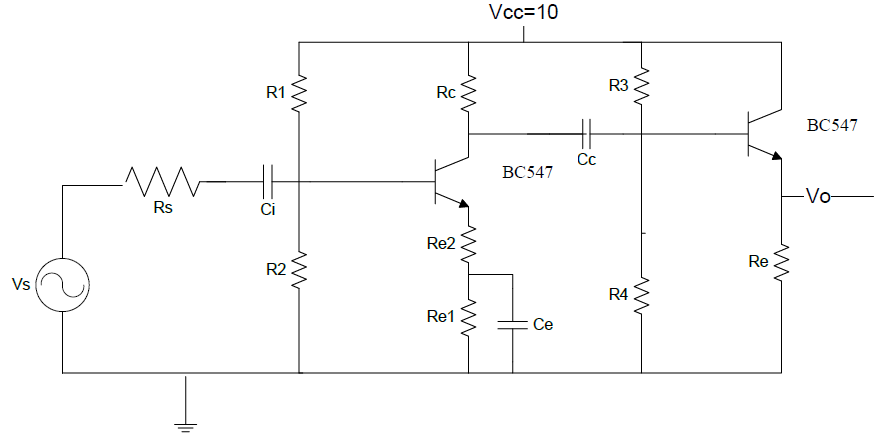
\includegraphics[width=\columnwidth]{schematic}
	\caption{Overall schematic of the multi-stage amplifier (adapted from \ref{ref:cktdsn})}
	\label{fig:sch}
\end{figure}

\parskip=6pt
The transistor has a gain of 200. $V_s$ and $R_s$ modelled the input signal and source impedance, $C_i$ is the input coupling capacitor, together with bias resistors $R_1$, $R_2$, $R_e1$, $R_e2$, load resistor $R_c$, emitter decoupling capacitor $C_e$, output coupling capacitor $C_c$ and transistor 1 created the first stage. Bias resistors $R_3$, $R_4$, $R_e$ and transistor 2 created the second stage.
\parskip=10pt

% Second stage design

\fontHeading
\stepcounter{sections}
\textbf{\arabic{sections}.\tab Second stage design}

\fontBody
The common collector stage was designed first.

\fontSubHeading
\stepcounter{subsections}
\textbf{\arabic{sections}.\arabic{subsections}\tab Choose collector current}
\parskip=6pt

\fontBody
Equation (\ref{eq:cc_ic}) from basic characteristic of BJTs states for a smaller collector current, base current would also be smaller. And the base current should not affect the base voltage bias, as in relationship (\ref{eq:cc_ir34}), $R_3$ and $R_4$ can be bigger for smaller base current, results in a larger input impedance. Therefore a small collector current of about $1mA$ should be appropriate.
\parskip=0pt

\begin{gather}
	I_c = \beta I_b
	\label{eq:cc_ic}\\
	I_{R_{3,4}} \gg I_{b2}
	\label{eq:cc_ir34}
\end{gather}
\parskip=6pt

\fontSubHeading
\stepcounter{subsections}
\textbf{\arabic{sections}.\arabic{subsections}\tab Determine output quiescent point}

\fontBody
From basic equation (\ref{eq:cc_ie}) of BJTs, for a small $I_b$, $I_e$ was approximately the same as $I_c$.
\parskip=0pt

\begin{equation}
	I_e = I_c + I_b = \left( 1 + \beta \right) I_b
	\label{eq:cc_ie}
\end{equation}
\parskip=6pt

As show in the schematic Figure \ref{fig:sch}, using KVL, $R_e$ is related to $I_{c2}$ by equation (\ref{eq:cc_re}).
\parskip=0pt

\begin{gather}
	V_{cc} = V_{CE2} + I_{e2} R_e \nonumber \\
	R_e = \frac{V_{cc} - V_{CE2}}{I_{e2}} \approx \frac{V_{cc} - V_{CE2}}{I_{c2}}
	\label{eq:cc_re}
\end{gather}
\parskip=6pt

From transistor BC547 datasheet, $V_{BE2} = 0.66V$ at $I_{c2} = 1mA$. Therefore to have full output swing at $V_{B2}$ and $V_{E2}$, the average of these two voltages should be $\frac{Vcc}{2}$ as in equation (\ref{eq:cc_ve2}).
\parskip=0pt

\begin{gather}
	\frac{V_{B2} + V_{E2}}{2} = \frac{V_{cc}}{2} \nonumber \\
	V_{E2} = \frac{V_{cc} - V_{BE}}{2} \approx 4.67V
	\label{eq:cc_ve2}
\end{gather}
\parskip=6pt

\fontSubHeading
\stepcounter{subsections}
\textbf{\arabic{sections}.\arabic{subsections}\tab Choose resistor $R_e$}

By Ohm’s law, $R_e$ could be calculated as in equation (\ref{eq:cc_reR}).
\parskip=0pt

\begin{equation}
	R_e = \frac{V_{E2}}{I_{e2}} \approx 4.67k\Omega
	\label{eq:cc_reR}
\end{equation}
\parskip=6pt

For standard E12 series resistors, choose $R_e = 4.7k\Omega$.

\fontSubHeading
\stepcounter{subsections}
\textbf{\arabic{sections}.\arabic{subsections}\tab Determine bias resistor R3 and R4}

Base current $I_{b2}$ must not affect bias voltage determined by $R_3$ and $R_4$, as in equation (\ref{eq:cc_ir34size}).
\parskip=0pt

\begin{gather}
	I_{b2} = \frac{I_{e2}}{\beta + 1} = \frac{V_{E2}}{R_e\left(\beta + 1\right)} \approx 4.94\mu A \nonumber \\
	I_{R_{3,4}} > 10 I_{b2} \approx 49.4\mu A \gg I_{b2}
	\label{eq:cc_ir34size}
\end{gather}
\parskip=6pt

Apply KVL as in equation (\ref{eq:cc_ir34}) and bias conditions as (\ref{eq:cc_r4}), $R_4$ chosen to be $100k\Omega$ in E12 series, while $R_3$ calculated as in (\ref{eq:cc_r3}) to be $82k\Omega$.
\parskip=0pt

\begin{gather}
	\label{eq:cc_ir34}
	I_{R_{3,4}} = \frac{V_{cc}}{R_3 + R_4} \\
	V_{B2} = V_{E2} + V_{BE} \approx 5.33 \nonumber \\
	\label{eq:cc_r4}
	R_4 = \frac{V_{B2}}{I_{R_{3,4}}} \approx 108k\Omega \\
	\label{eq:cc_r3}
	R_3 = \frac{V_{cc} - V_{B2}}{I_{R_{3,4}}} \approx 94.5k\Omega
\end{gather}
\parskip=6pt

\fontSubHeading
\stepcounter{subsections}
\textbf{\arabic{sections}.\arabic{subsections}\tab Estimate gain, input impedance and output impedance}

To estimate these parameters, use hybrid pi small signal model shown in Figure \ref{fig:cc_small}.
\parskip=0pt

\begin{figure}[H]
	\centering
	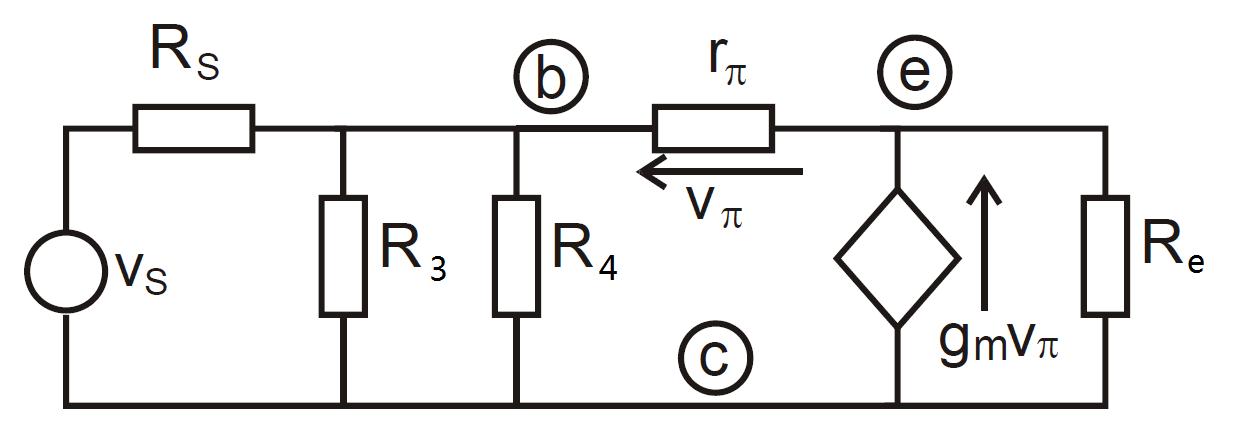
\includegraphics[width=\columnwidth]{cc_small}
	\caption{Small signal model of common collector stage (adapted from \ref{ref:sli_b})}
	\label{fig:cc_small}
\end{figure}

For simplicity, consider $V_B$ as input voltage, $R_{in}$ as input resistance from $V_B$, $R_{in}$, $R_3$, $R_4$ and $R_s$ form a potential divider described by equation (\ref{eq:cc_vb}).
\parskip=0pt

\begin{gather}
	R_i = \left( \frac{1}{R_3} + \frac{1}{R_4} + \frac{1}{R_{in}} \right)^{-1} \nonumber \\
	V_B = V_S\frac{R_i}{R_i + R_S}
	\label{eq:cc_vb}
\end{gather}
\parskip=6pt

By using BJT characteristic $r_\pi$ described by (\ref{eq:cc_gm}) and KCL analysis at emitter described by (\ref{eq:cc_kcl}):
\parskip=0pt

\begin{gather}
	\label{eq:cc_gm}
	r_\pi = \frac{\beta}{g_m} \\
	\label{eq:cc_kcl}
	g_m \left( V_E - V_B \right) + \frac{V_E - V_B}{r_\pi} + \frac{V_E}{R_e} = 0
\end{gather}
\parskip=6pt

Equation for gain (\ref{eq:cc_gain}) and input impedance (\ref{eq:cc_rin}) can be therefore analysed:
\parskip=0pt

\begin{gather}
	\label{eq:cc_gain}
	A = \frac{V_E}{V_S} = \frac{R_i}{R_i + R_S}\frac{V_E}{V_B} = \frac{R_i}{R_i + R_S}\frac{R_e\left( 1 + \beta \right)}{r_\pi + R_e\left( 1 + \beta \right)} \\
	I_b = \frac{V_B - V_E}{r_\pi} = \frac{V_B}{r_\pi + R_e\left( 1 + \beta \right)} \nonumber \\
	R_{in} = \frac{V_B}{I_b} = r_\pi + R_e(1 + \beta) \nonumber \\
	\label{eq:cc_rin}
	R_i = \left( \frac{1}{R_3} + \frac{1}{R_4} + \frac{1}{r_\pi + R_e\left( 1 + \beta \right)}\right) ^{-1}
\end{gather}
\parskip=6pt

Calculate $g_m$ and $r_\pi$ from $I_c$:
\parskip=0pt

\begin{gather}
	\label{eq:gm}
	g_m = \frac{q I_c}{k T} \approx 38.6 I_c \\
	\label{eq:rpi}
	r_\pi = \frac{\beta}{g_m} \approx \frac{5.175}{I_c} \approx 5.2k\Omega
\end{gather}
\parskip=6pt

Use source impedance for function generator $R_S \approx 50\Omega$, put values in equation for gain (\ref{eq:cc_gain}): $A \approx 0.99$, input impedance (\ref{eq:cc_rin}): $R_i \approx 43k\Omega$.

To calculate output impedance, consider a current source at output and the impact of the circuit on the current source as in Figure \ref{fig:cc_rout}, where $R_S' = R_S \| R_3 \| R_4$.
\parskip=0pt

\begin{figure}[H]
	\centering
	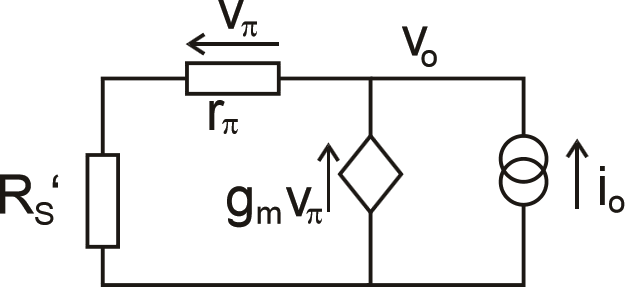
\includegraphics[width=\columnwidth]{cc_rout}
	\caption{Simplified small signal model of common collector for calculate output impedance (adapted from \ref{ref:sli_b})}
	\label{fig:cc_rout}
\end{figure}
\parskip=6pt

Solving the system described by KCL analysis at emitter (\ref{eq:cc_rout_kcl}), $V_\pi$ from potential divider (\ref{eq:cc_rout_vpi}):
\parskip=0pt

\begin{gather}
	\label{eq:cc_rout_kcl}
	i_o + g_m V_\pi - \frac{V_o}{R_S' + r_\pi} = 0 \\
	\label{eq:cc_rout_vpi}
	V_\pi = -\frac{V_o r_\pi}{R_S' + r_\pi}
\end{gather}
\parskip=6pt

Output impedance can be therefore analysed by (\ref{eq:cc_rout}).
\parskip=0pt

\begin{equation}
	\label{eq:cc_rout}
	R_o = \frac{V_o}{I_o} = \frac{R_S' + r_\pi}{1 + \beta}
\end{equation}
\parskip=6pt

Use source impedance for function generator $R_S \approx 50\Omega$, put values in equation for output impedance: $R_o \approx 26.1\Omega$.
\parskip=10pt

% First stage design

\fontHeading
\stepcounter{sections}
\textbf{\arabic{sections}.\tab First stage design}

\fontBody
The common emitter stage need to be designed after common collector stage, because in order to avoid loading between two stages, output impedance of common emitter stage should be much less than input impedance of common collector stage as described by (\ref{eq:ce_routrelat}).
\parskip=0pt

\begin{equation}
	\label{eq:ce_routrelat}
	R_{o1} < \frac{R_{in2}}{10} \approx 4.3k\Omega
\end{equation}
\parskip=6pt

\fontSubHeading
\stepcounter{subsections}
\textbf{\arabic{sections}.\arabic{subsections}\tab Determine load resistor $R_c$}

\fontBody
The load resistor $R_c$ of common emitter stage equals to the output impedance, so choose $R_c = 3.9k\Omega$.

\fontSubHeading
\stepcounter{subsections}
\textbf{\arabic{sections}.\arabic{subsections}\tab Estimate gain and input impedance}

To estimate these parameters, use hybrid pi small signal model shown in Figure \ref{fig:ce_small}.
\parskip=0pt

\begin{figure}[H]
	\centering
	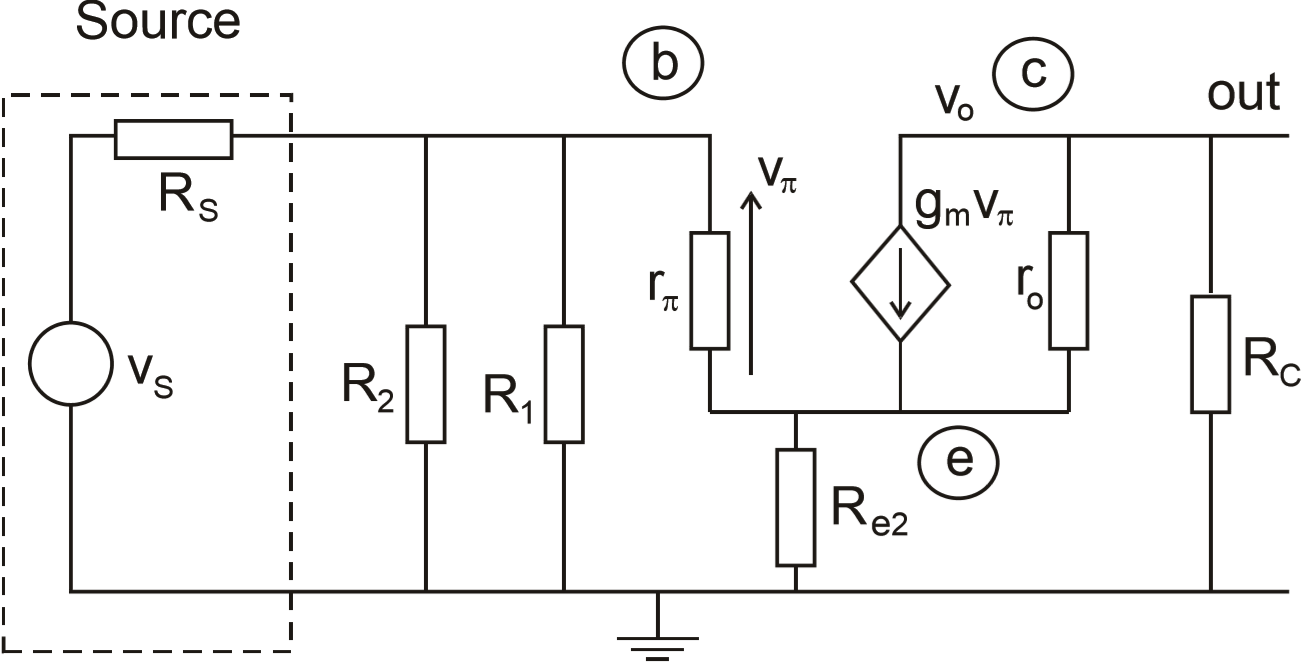
\includegraphics[width=\columnwidth]{ce_small}
	\caption{Small signal model of common emitter stage (adapted from \ref{ref:sli_a})}
	\label{fig:ce_small}
\end{figure}
\parskip=6pt

Solving the system described by KVL analysis of $V_c$ (\ref{eq:ce_kvl_vc}), KCL analysis at emitter (\ref{eq:ce_kcl_e}), gain can be descibed as (\ref{eq:ce_gain}).
\parskip=0pt

\begin{gather}
	\label{eq:ce_kvl_vc}
	V_c = -g_m \left(V_b - V_e\right) R_c
	\\\label{eq:ce_kcl_e}
	\frac{V_e}{R_{e2}} + \frac{V_e - V_b}{r_\pi} - g_m\left(V_b - V_e\right) = 0
	\\\label{eq:ce_gain}
	A = \frac{V_c}{V_b} = \frac{-\beta R_c}{r_\pi + R_{e2}\left( 1 + \beta \right)}
\end{gather}
\parskip=6pt

If $R_{e2}\beta$ is large, gain can be approximated by (\ref{eq:ce_gain_approx}).
\parskip=0pt

\begin{equation}
	\label{eq:ce_gain_approx}
	A \approx -\frac{R_c}{R_{e2}}
\end{equation}
\parskip=6pt

Equation (\ref{eq:ce_rinb}) described input impedance at base terminal:
\parskip=0pt

\begin{equation}
	\label{eq:ce_rinb}
	R_b = \frac{V_b}{I_b} = \frac{V_b}{\frac{V_b - V_e}{r_\pi}} = r_\pi + R_{e2}\left( 1 + \beta \right)
\end{equation}
\parskip=6pt

Therefore total input impedance can be described as (\ref{eq:ce_rin}).
\parskip=0pt

\begin{equation}
	\label{eq:ce_rin}
	R_{in} = R_1 \| R_2 \| R_b = \left(\frac{1}{R_1} + \frac{1}{R_2} + \frac{1}{r_\pi + R_{e2}\left( 1 + \beta \right)}\right)^{-1}
\end{equation}
\parskip=6pt

\fontSubHeading
\stepcounter{subsections}
\textbf{\arabic{sections}.\arabic{subsections}\tab Determine bias resistor $R_{e2}$}

Had determined $R_{o1} = R_c = 3.9k\Omega$, gain of common collector stage should be approximately $0.91$.

Desired gain is $6$, so common emitter stage should have a gain of approximately $6.59$.

By solving equation (\ref{eq:ce_gain_approx}), $R_{e2} \approx 592\Omega$, choose $R_{e2} = 560\Omega$.

\fontSubHeading
\stepcounter{subsections}
\textbf{\arabic{sections}.\arabic{subsections}\tab Determine bias resistor $R_{e1}$ and $V_{CE1}$}

To have maximum swing at the output of the common emitter stage, $V_{C1} = \frac{V_{cc}}{2} = 5V$.

Therefore collector current $I_{c1}$ can be determined by (\ref{eq:ce_ic1}).
\parskip=0pt

\begin{equation}
	\label{eq:ce_ic1}
	I_{c1} = \frac{V_{cc} - V_{C1}}{R_c} \approx 1.28mA
\end{equation}
\parskip=6pt

Choose $R_{e1}$ to be $470\Omega$, $V_{CE}$ can be therefore determined by (\ref{eq:ce_vce}) using KVL.
\parskip=0pt

\begin{gather}
	I_{e1} = I_{c1} \left( 1 + \frac{1}{\beta} \right) \approx 1.29mA \nonumber \\
	\label{eq:ce_vce}
	V_{CE1} = V_{C} - I_{e1} \left( R_{e1} + R_{e2} \right) \approx 3.67V
\end{gather}
\parskip=6pt

\fontSubHeading
\stepcounter{subsections}
\textbf{\arabic{sections}.\arabic{subsections}\tab Determine bias resistors $R_1$ and $R_2$}

Solving bias condition described by $V_{B1}$ (\ref{eq:ce_vb1}), input impedance specification (\ref{eq:ce_rinspec}), potential divider (\ref{eq:ce_r1r2}):
\parskip=0pt

\begin{gather}
	\label{eq:ce_vb1}
	V_{B1} = V_{C1} - V_{CE1} \approx 1.33V \\
	r_\pi \approx 4.04k\Omega \nonumber \\
	\label{eq:ce_rinspec}
	R_{in} = \left(\frac{1}{R_1} + \frac{1}{R_2} + \frac{1}{r_\pi + R_{e2}\left( 1 + \beta \right)}\right)^{-1} \leq 40k\Omega\\
	\label{eq:ce_r1r2}
	\frac{V_{B1}}{V_{cc}} = \frac{R_2}{R_1 + R_2}
\end{gather}
\parskip=6pt

In E12 series, choose $R_1 = 390k\Omega$ and $R_2 = 100k\Omega$.

\fontSubHeading
\stepcounter{subsections}
\textbf{\arabic{sections}.\arabic{subsections}\tab Determine emitter decoupling capacitor $C_e$}

%Apply equation (\ref{eq:ce_ce}), choose $f = \SI{1}{\kilo\hertz}$, $C_e \geq \SI{5.02}{\micro\farad}$.
Apply equation (\ref{eq:ce_ce}), choose $f = 1$kHz, $C_e \geq 5.02\mu$F.
\parskip=0pt

\begin{equation}
	\label{eq:ce_ce}
	C_e \geq \frac{10}{2\pi f\left(R_{e1} \| \left(R_{e2} + \frac{r_{\pi 1}}{\beta + 1} + \frac{R_1 \| R_2}{\beta + 1}\right)\right)}
\end{equation}
\parskip=6pt

\fontSubHeading
\stepcounter{subsections}
\textbf{\arabic{sections}.\arabic{subsections}\tab Determine input coupling capacitor $C_i$}

%Apply equation (\ref{eq:ce_ci}), choose $f = \SI{1}{\kilo\hertz}$, $R_S = 50\Omega$ from function generator, $C_i \geq \SI{33.6}{\nano\farad}$.
Apply equation (\ref{eq:ce_ci}), choose $f = 1$kHz, $R_S = 50\Omega$ from function generator, $C_i \geq 33.6$nF.
\parskip=0pt

\begin{equation}
	\label{eq:ce_ci}
	C_i \geq \frac{10}{2\pi f\left(R_S + R_1 \| R_2 \| \left(r_{\pi1} + \left(\beta + 1\right)R_{e2}\right)\right)}
\end{equation}
\parskip=10pt

% Multi stage design

\fontHeading
\stepcounter{sections}
\textbf{\arabic{sections}.\tab Multi-stage design}

\fontBody
The overall gain of multi-stage amplifier calculated from equation (\ref{eq:cc_gain}) and equation (\ref{eq:ce_gain}) is $-6.10$, within specification.
\parskip=6pt

The overall input impedance of multi-stage amplifier from equation (\ref{eq:ce_rinspec}) is $47k\Omega$, within specification.

The overall output impedance of multi-stage amplifier from $R_{o1} = R_c$ and equation (\ref{eq:cc_rout}) is $43\Omega$, within specification.
\parskip=10pt

% Simulation

\fontHeading
\stepcounter{sections}
\textbf{\arabic{sections}.\tab SPICE simulation}

\fontBody
After determined the parameters of components, the circuit was simulated by using LTspice software.
\parskip=6pt

Quiescent voltage analysed from simulation as shown in Figure \ref{fig:simulation}, there were some difference from calculated value, but still acceptable.
\parskip=0pt

\begin{figure}[H]
	\centering
	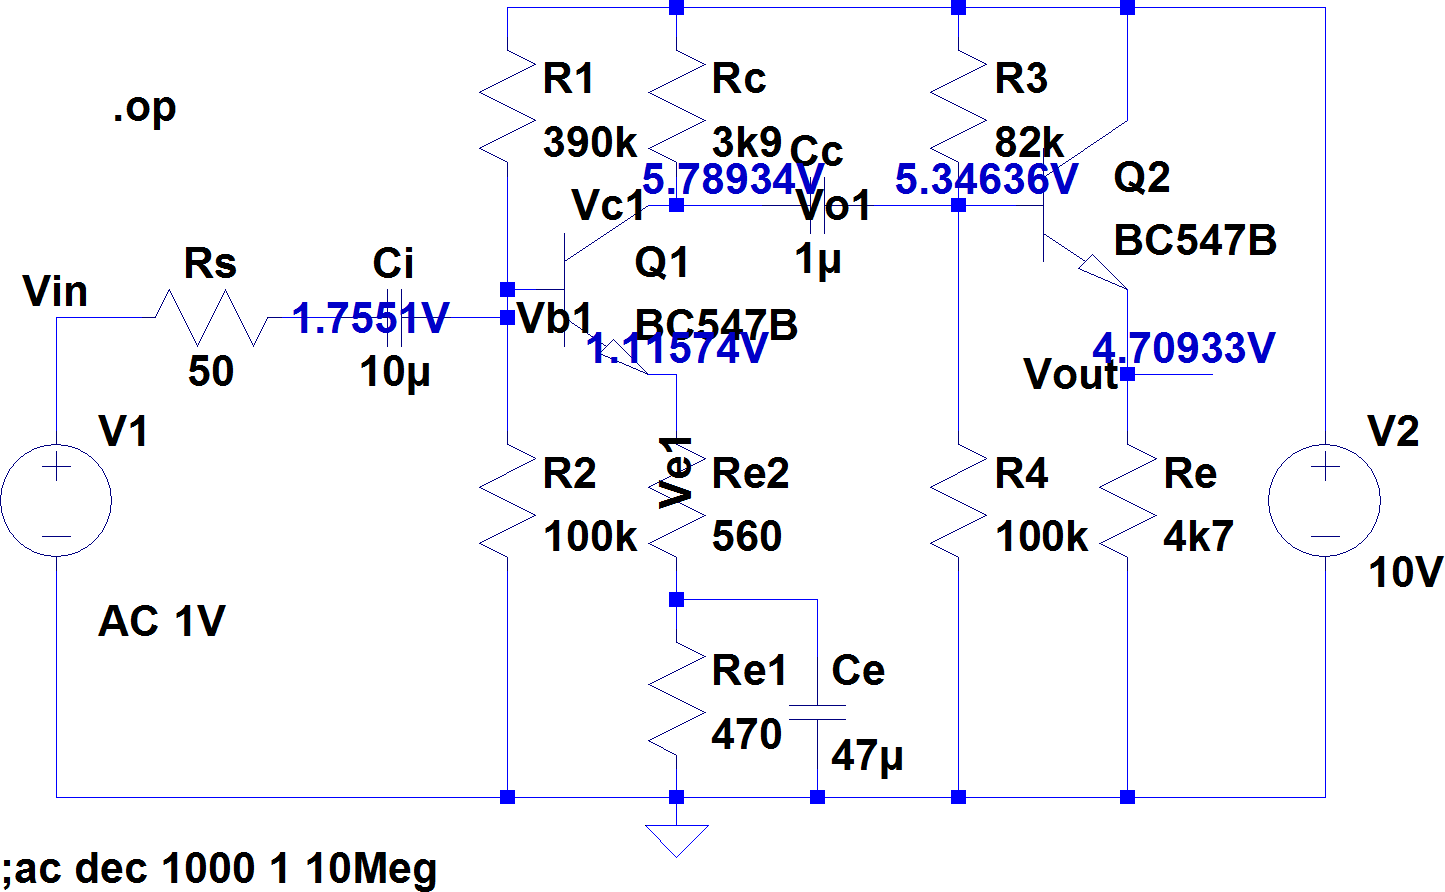
\includegraphics[width=0.8\columnwidth]{simulation}
	\caption{LTspice operation point analysis of multi-stage amplifier}
	\label{fig:simulation}
\end{figure}
\parskip=6pt

Frequency response analysed from simulation as shown in Figure \ref{fig:freq}, mind-band gain was $6.04$, bandwidth was $10.7$MHz.
\parskip=0pt

\begin{figure}[H]
	\centering
	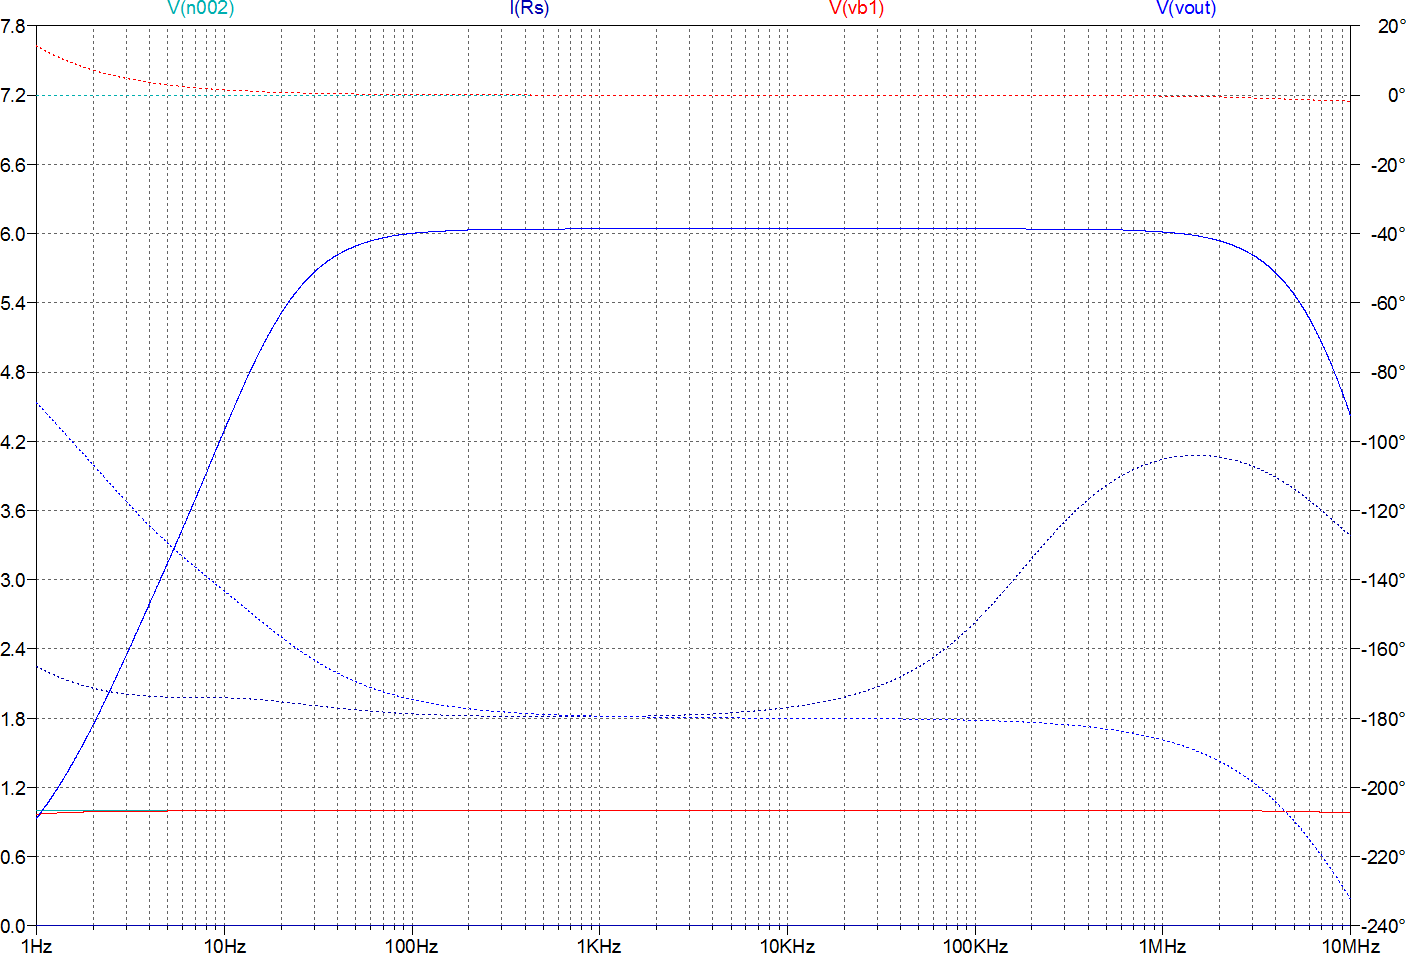
\includegraphics[width=0.8\columnwidth]{freq}
	\caption{LTspice frequency response analysis of multi-stage amplifier}
	\label{fig:freq}
\end{figure}
\parskip=10pt

% Laboratory work

\fontHeading
\stepcounter{sections}
\textbf{\arabic{sections}.\tab Laboratory work}

\parskip=6pt
\fontSubHeading
\stepcounter{subsections}
\textbf{\arabic{sections}.\arabic{subsections}\tab Measuring gain}

Mid-band gain can be easily measured by setup a function generator at input terminal, in sine wave mode with mid-band frequency (e.g. $f = 1$kHz), then use an oscilloscope to measure the amplitude of output signal voltage, gain $A = \frac{V_{out}}{V_{in}}$.

\fontSubHeading
\stepcounter{subsections}
\textbf{\arabic{sections}.\arabic{subsections}\tab Measuring input impedance}

Input impedance can be measured by connect a potentiometer in series with input terminal as shown in Figure \ref{fig:inputimp}, then adjust the potentiometer until amplitude of signal at input terminal become half of original signal, the input resistance is approximately the same as the resistance of the potentiometer.
\parskip=0pt

\begin{figure}[H]
	\centering
	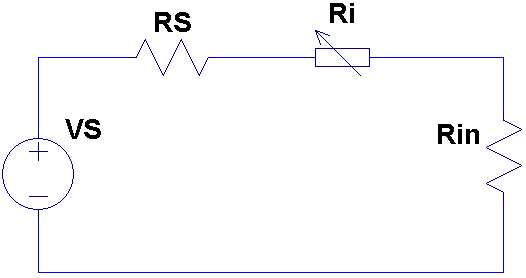
\includegraphics[width=\columnwidth]{inputimp}
	\caption{Input impedance measuring}
	\label{fig:inputimp}
\end{figure}
\parskip=6pt

\fontSubHeading
\stepcounter{subsections}
\textbf{\arabic{sections}.\arabic{subsections}\tab Measuring output impedance}

Output impedance can be measured at the same way, by connect a load potentiometer at output terminal as shown in Figure \ref{fig:outputimp}, then adjust the potentiometer until amplitude of signal at output terminal become half of original signal, the output resistance is approximately the same as the resistance of the potentiometer.
\parskip=0pt

\begin{figure}[H]
	\centering
	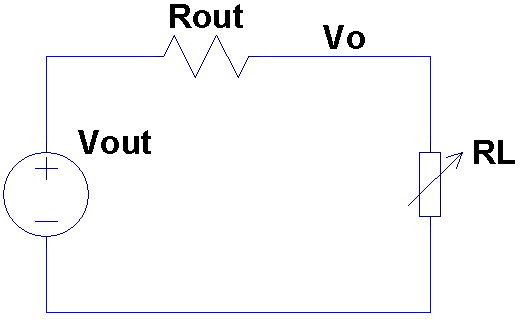
\includegraphics[width=\columnwidth]{outputimp}
	\caption{Output impedance measuring}
	\label{fig:outputimp}
\end{figure}
\parskip=6pt

\fontSubHeading
\stepcounter{subsections}
\textbf{\arabic{sections}.\arabic{subsections}\tab Measuring quiescent point}

\fontBody
Quiescent voltage was measured firstly, as shown in Table \ref{tb:qv}, not much difference from simulation values.
\parskip=0pt\par
\sepTable
\begin{table}[H]
\caption{Quiescent voltage measured in laboratory}
\label{tb:qv}
\begin{nscenter}
\begin{tabular}{c | c | c}
	\hline
	Voltage & Simulation & Measurement \\ \hline
	Vc1	& 5.789	& 5.71	\\
	Vb1	& 1.755	& 1.766	\\
	Ve1	& 1.116	& 1.132	\\
	Vc2	& 10	& 9.99	\\
	Vb2	& 5.346	& 5.34	\\
	Ve2	& 4.709	& 4.72	\\ \hline
\end{tabular}
\end{nscenter}
\end{table}
\sepFigure
\parskip=6pt

\fontSubHeading
\stepcounter{subsections}
\textbf{\arabic{sections}.\arabic{subsections}\tab Measuring first stage}

By using the method described above, the mid-band gain of first stage as shown in Figure \ref{fig:lab_ce_gain}, was $A \approx \frac{6.60}{1.02} = 6.47$.
\parskip=0pt

\begin{figure}[H]
	\centering
	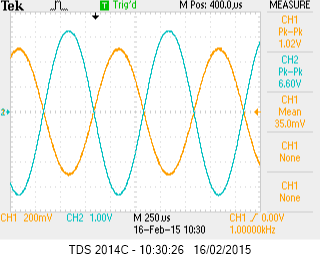
\includegraphics[width=0.85\columnwidth]{labcegain}
	\caption{Mid-band gain measurement of first stage, oscilloscope screen capture of input signal at CH1, output signal at CH2}
	\label{fig:lab_ce_gain}
\end{figure}
\parskip=6pt

The input impedance is $R_{in} \approx R_i = 60.1k\Omega$, when input signal amplitude became half the signal from function generator as shown in Figure \ref{fig:lab_ce_rin}.
\parskip=0pt

\begin{figure}[H]
	\centering
	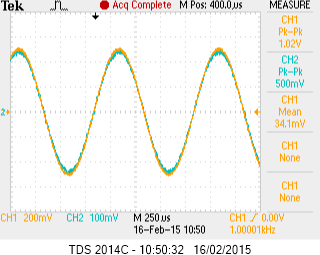
\includegraphics[width=0.85\columnwidth]{labcerin}
	\caption{Input impedance measurement of first stage, oscilloscope screen capture of half input signal amplitude}
	\label{fig:lab_ce_rin}
\end{figure}
\parskip=6pt

The output impedance is $R_{out} \approx R_L = 3.84k\Omega$, when output signal amplitude became half the original signal as shown in Figure \ref{fig:lab_ce_rout}.
\parskip=0pt

\begin{figure}[H]
	\centering
	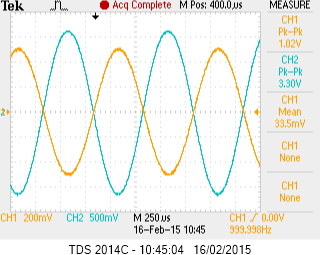
\includegraphics[width=0.85\columnwidth]{labcerout}
	\caption{Output impedance measurement of first stage, oscilloscope screen capture of half output signal amplitude from original output signal shown in Figure \ref{fig:lab_ce_gain}}
	\label{fig:lab_ce_rout}
\end{figure}
\parskip=6pt

By measuring voltage gain at different frequencies, the frequency response analysis can be plotted as shown in Figure \ref{fig:lab_ce_freq}, bandwidth $\approx 2$MHz.
\parskip=0pt

\begin{figure}[H]
	\centering
	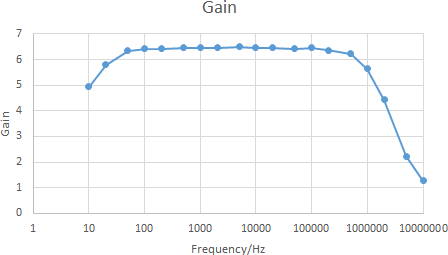
\includegraphics[width=0.85\columnwidth]{labcefreq}
	\caption{Frequency response analysis, produced from measuring voltage gain at different frequencies}
	\label{fig:lab_ce_freq}
\end{figure}
\parskip=6pt

Mid-band gain of first stage with $C_e$ removed measured as shown in Figure \ref{fig:lab_ce_gain_removed}, was $A \approx \frac{3.72}{1.02} = 3.65$. From equation (\ref{eq:ce_gain}), $R_{e2}$ become approximately doubled, therefore gain approximately halved.
\parskip=0pt

\begin{figure}[H]
	\centering
	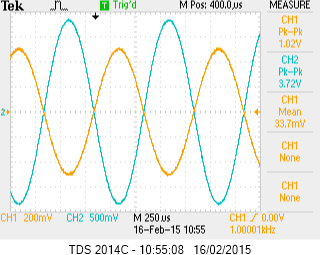
\includegraphics[width=0.85\columnwidth]{labcegainremoved}
	\caption{Mid-band gain measurement of first stage, after $C_e$ removed}
	\label{fig:lab_ce_gain_removed}
\end{figure}
\parskip=6pt

Mid-band gain of first stage with $C_e$ bypassed $R_{e1}$ and $R_{e2}$ measured as shown in Figure \ref{fig:lab_ce_gain_bridged}, was $A \approx \frac{7.20}{63.2\times 10^{-3}} = 114$. From equation (\ref{eq:ce_gain}), gain from transistor is only affected by $\frac{R_c}{R_{\pi1}} \approx 0.975$.
\parskip=0pt

\begin{figure}[H]
	\centering
	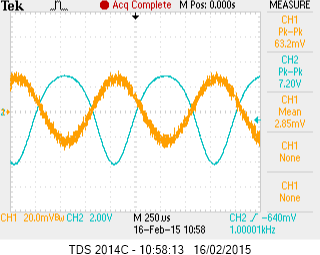
\includegraphics[width=0.85\columnwidth]{labcegainbridged}
	\caption{Mid-band gain measurement of first stage, after emitter resistance totally bypassed by $C_e$}
	\label{fig:lab_ce_gain_bridged}
\end{figure}
\parskip=6pt

\fontSubHeading
\stepcounter{subsections}
\textbf{\arabic{sections}.\arabic{subsections}\tab Measuring second stage}

By using the method described above, the mid-band gain of second stage as shown in Figure \ref{fig:lab_cc_gain}, was $A \approx \frac{5.00}{5.04} = 0.99$.
\parskip=0pt

\begin{figure}[H]
	\centering
	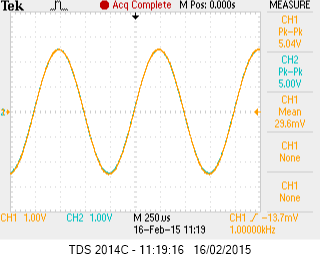
\includegraphics[width=0.85\columnwidth]{labccgain}
	\caption{Mid-band gain measurement of second stage, oscilloscope screen capture of input signal at CH1, output signal at CH2}
	\label{fig:lab_cc_gain}
\end{figure}
\parskip=6pt

The input impedance is $R_{in} \approx R_i = 44.7k\Omega$, when input signal amplitude became half the signal from function generator as shown in Figure \ref{fig:lab_cc_rin}.
\parskip=0pt

\begin{figure}[H]
	\centering
	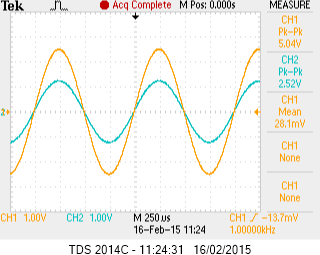
\includegraphics[width=0.85\columnwidth]{labccrin}
	\caption{Input impedance measurement of second stage, oscilloscope screen capture of half input signal amplitude}
	\label{fig:lab_cc_rin}
\end{figure}
\parskip=6pt

The output impedance is $R_{out} \approx R_L = 152.3\Omega$, when output signal amplitude became half the original signal as shown in Figure \ref{fig:lab_cc_rout}.
\parskip=0pt

\begin{figure}[H]
	\centering
	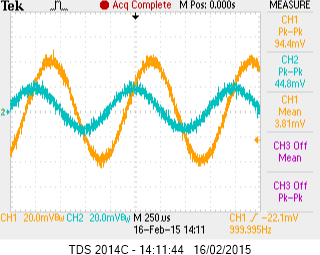
\includegraphics[width=0.85\columnwidth]{labccrout}
	\caption{Output impedance measurement of second stage, oscilloscope screen capture of half output signal amplitude from input signal (gain $\approx 1$)}
	\label{fig:lab_cc_rout}
\end{figure}
\parskip=6pt

\fontSubHeading
\stepcounter{subsections}
\textbf{\arabic{sections}.\arabic{subsections}\tab Measuring multi-stage amplifier}

By using the method described above, the mid-band gain of multi-stage stage as shown in Figure \ref{fig:lab_multi_gain}, was $A \approx \frac{6.04}{1.02} = 5.92$.
\parskip=0pt

\begin{figure}[H]
	\centering
	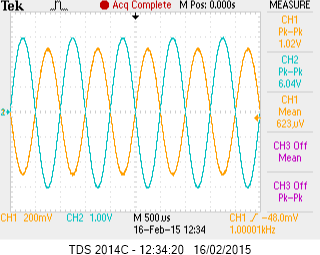
\includegraphics[width=0.85\columnwidth]{labmultigain}
	\caption{Mid-band gain measurement of multi-stage amplifier, oscilloscope screen capture of input signal at CH1, output signal at CH2}
	\label{fig:lab_multi_gain}
\end{figure}
\parskip=6pt

The input impedance is $R_{in} \approx R_i = 60.0k\Omega$, when input signal amplitude became half the signal from function generator as shown in Figure \ref{fig:lab_multi_rin}.
\parskip=0pt

\begin{figure}[H]
	\centering
	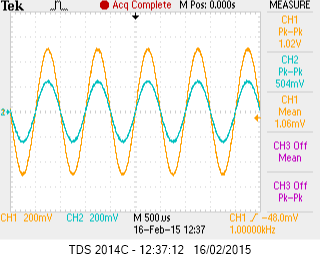
\includegraphics[width=0.85\columnwidth]{labmultirin}
	\caption{Input impedance measurement of multi-stage amplifier, oscilloscope screen capture of half input signal amplitude}
	\label{fig:lab_multi_rin}
\end{figure}
\parskip=6pt

To avoid clipping, the amplitude of input signal reduced as in Figure \ref{fig:lab_multi_gain_small}.
\parskip=0pt

\begin{figure}[H]
	\centering
	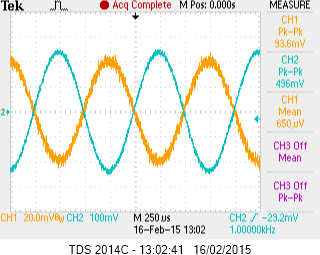
\includegraphics[width=0.85\columnwidth]{labmultigainsmall}
	\caption{Mid-band gain measurement of multi-stage amplifier, at reduced input signal amplitude}
	\label{fig:lab_multi_gain_small}
\end{figure}
\parskip=6pt

The output impedance is $R_{out} \approx R_L = 180.1\Omega$, when output signal amplitude became half the original signal as shown in Figure \ref{fig:lab_multi_rout}.
\parskip=0pt

\begin{figure}[H]
	\centering
	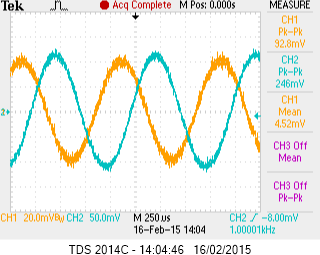
\includegraphics[width=0.85\columnwidth]{labmultirout}
	\caption{Output impedance measurement of multi-stage amplifier, oscilloscope screen capture of half output signal amplitude from original output signal shown in Figure \ref{fig:lab_multi_gain_small}}
	\label{fig:lab_multi_rout}
\end{figure}
\parskip=10pt

% Reflection

\fontHeading
\stepcounter{sections}
\textbf{\arabic{sections}.\tab Reflection}

\parskip=6pt
\fontBody
There were some differences in values of quiescent voltage, gain, input and output impedance from calculated, simulation and measured values, but still acceptable. And the overall gain $A = 5.92 \approx 6$, input impedance $R_{in} = 60.0k\Omega > 40k\Omega$ and output impedance $R_{out} = 180.1\Omega < 1.3k\Omega$ were all within the specifications, therefore the design was succeed.
\parskip=10pt

\fontHeading
\textbf{References}

\fontRef
\begin{enumerate}[label={[\arabic*]},align=left,leftmargin=0.7cm,labelwidth=!,topsep=0pt,partopsep=0pt,parsep=0pt,itemsep=0pt]
\item
\label{ref:cktdsn}
Sasan Mahmodi "Circuit Design" [\textit{Online}]. Available: \url{https://secure.ecs.soton.ac.uk/notes/elec2205/D3/d3coursework2.pdf}
\item
\label{ref:sli_a}
Peter Wilson "Lecture slides A" [\textit{Online}]. Available: \url{https://secure.ecs.soton.ac.uk/notes_so/elec2216/notes/elec2216_slides_1.pdf}
\item
\label{ref:sli_b}
Peter Wilson "Lecture slides B" [\textit{Online}]. Available: \url{https://secure.ecs.soton.ac.uk/notes_so/elec2216/notes/elec2216_slides_2.pdf}
\end{enumerate}
\end{multicols}

\end{document}
